% Options for packages loaded elsewhere
\PassOptionsToPackage{unicode}{hyperref}
\PassOptionsToPackage{hyphens}{url}
%
\documentclass[
]{article}
\usepackage{lmodern}
\usepackage{amssymb,amsmath}
\usepackage{ifxetex,ifluatex}
\ifnum 0\ifxetex 1\fi\ifluatex 1\fi=0 % if pdftex
  \usepackage[T1]{fontenc}
  \usepackage[utf8]{inputenc}
  \usepackage{textcomp} % provide euro and other symbols
\else % if luatex or xetex
  \usepackage{unicode-math}
  \defaultfontfeatures{Scale=MatchLowercase}
  \defaultfontfeatures[\rmfamily]{Ligatures=TeX,Scale=1}
\fi
% Use upquote if available, for straight quotes in verbatim environments
\IfFileExists{upquote.sty}{\usepackage{upquote}}{}
\IfFileExists{microtype.sty}{% use microtype if available
  \usepackage[]{microtype}
  \UseMicrotypeSet[protrusion]{basicmath} % disable protrusion for tt fonts
}{}
\makeatletter
\@ifundefined{KOMAClassName}{% if non-KOMA class
  \IfFileExists{parskip.sty}{%
    \usepackage{parskip}
  }{% else
    \setlength{\parindent}{0pt}
    \setlength{\parskip}{6pt plus 2pt minus 1pt}}
}{% if KOMA class
  \KOMAoptions{parskip=half}}
\makeatother
\usepackage{xcolor}
\IfFileExists{xurl.sty}{\usepackage{xurl}}{} % add URL line breaks if available
\IfFileExists{bookmark.sty}{\usepackage{bookmark}}{\usepackage{hyperref}}
\hypersetup{
  hidelinks,
  pdfcreator={LaTeX via pandoc}}
\urlstyle{same} % disable monospaced font for URLs
\usepackage{graphicx}
\makeatletter
\def\maxwidth{\ifdim\Gin@nat@width>\linewidth\linewidth\else\Gin@nat@width\fi}
\def\maxheight{\ifdim\Gin@nat@height>\textheight\textheight\else\Gin@nat@height\fi}
\makeatother
% Scale images if necessary, so that they will not overflow the page
% margins by default, and it is still possible to overwrite the defaults
% using explicit options in \includegraphics[width, height, ...]{}
\setkeys{Gin}{width=\maxwidth,height=\maxheight,keepaspectratio}
% Set default figure placement to htbp
\makeatletter
\def\fps@figure{htbp}
\makeatother
\setlength{\emergencystretch}{3em} % prevent overfull lines
\providecommand{\tightlist}{%
  \setlength{\itemsep}{0pt}\setlength{\parskip}{0pt}}
\setcounter{secnumdepth}{-\maxdimen} % remove section numbering

\author{}
\date{}

\begin{document}

\# chapter 11

\hypertarget{header-n2}{%
\subsection{实验11}\label{header-n2}}

\hypertarget{header-n3}{%
\subsubsection{code}\label{header-n3}}

\begin{verbatim}
assume cs:code,ds:data

data segment
    db "Beginner's All-purpose Symbolic Instruction Code.",0
data ends


code segment
start:
    mov ax,data
    mov ds,ax
    mov si,0
	mov di,160*10+2*5

    call show_letter
    call letterc
	add di,160
    call show_letter

    mov ax,4c00h
    int 21h

    letterc:
        push ax
        push bx
        push cx
        push dx
        push si
        push di
        push ds
        push es

        mov si,0

    letterc_bg:
        mov al,ds:[si]

        cmp al,0
        je letterc_end

        cmp al,'a'
		jb next
		cmp al,'z'
		ja next
		;and al,11011111b
        sub al,20h
		mov ds:[si],al

        next:
            inc si
            jmp letterc_bg
    letterc_end:
        pop es
        pop ds
        pop di
        pop si
        pop dx
        pop cx
        pop bx
        pop ax
        ret

    show_letter:
        push ax
        push bx
        push cx
        push dx
        push si
        push di
        push ds
        push es
    show_letter_bg:
        mov ax,0b800h
        mov es,ax
        ; mov di,160*10+2*5

		mov cx,0

        show:
            mov al,ds:[si]

            mov cl,al
			jcxz show_letter_end
            
            mov ah,2
            mov es:[di],ax
            inc si
            inc di
            inc di
            jmp show

    show_letter_end:
        pop es
        pop ds
        pop di
        pop si
        pop dx
        pop cx
        pop bx
        pop ax
        ret
code ends
end start
\end{verbatim}

\hypertarget{header-n5}{%
\subsubsection{Screenshot}\label{header-n5}}

\begin{figure}
\centering
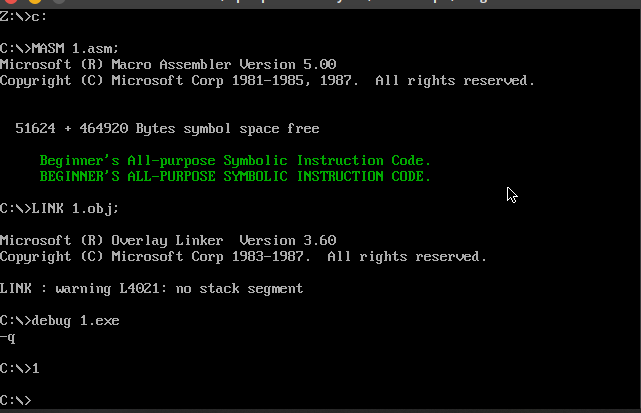
\includegraphics{/home/shenxin/workspace/ASM/实验文档/chapter11/chapter11.assets/Screenshot_20200317_104459.png}
\caption{}
\end{figure}

\end{document}
